\documentclass{article}
\usepackage{shoot}
%\usepackage[margin=0.25cm,usletter,landscape]{geometry}

\begin{document}

\begin{figure}
    \centering
	\vspace{0.01cm}
	\resizebox{\textwidth}{!}{%	
    % to plot timeseries.dat in table format
    \pgfplotstableread{time.dat}\loadedtable
    
    \begin{tikzpicture}
    	\begin{axis}[
    		ymin=0,
    		%minor tick num=4,
    		const plot,
    		%axis on top,
    		stack plots=y,
    		area style,
    		enlarge x limits = false,
    		cycle list={%
    			{blue!70!black,fill=blue},%
    			{blue!60!white,fill=blue!30!white},%
    			{draw=none,fill={rgb:red,138;green,82;blue,232}},%
    			{red,thick}%
    		},
    		legend style={
    			area legend,
    			at={(-0.5,1)},
    			anchor=west,
    			legend columns=2}]
    
    	\addplot table[x=time,y=memused]      from \loadedtable \closedcycle;
    	\addplot table[x=time,y=memcached]    from \loadedtable \closedcycle;
    	\addplot table[x=time,y=membuf]       from \loadedtable \closedcycle;
    	\addplot+[stack plots=false]
    			 table[x=time,y=memtotal]     from \loadedtable;
    	\legend{Manage,Sell,Freight,Optimal}
    	\end{axis}
    \end{tikzpicture}
    
    %\pgfplotstableread{time.dat}\loadedtable
    %\pgfplotstabletypeset\loadedtable
    
    
    
    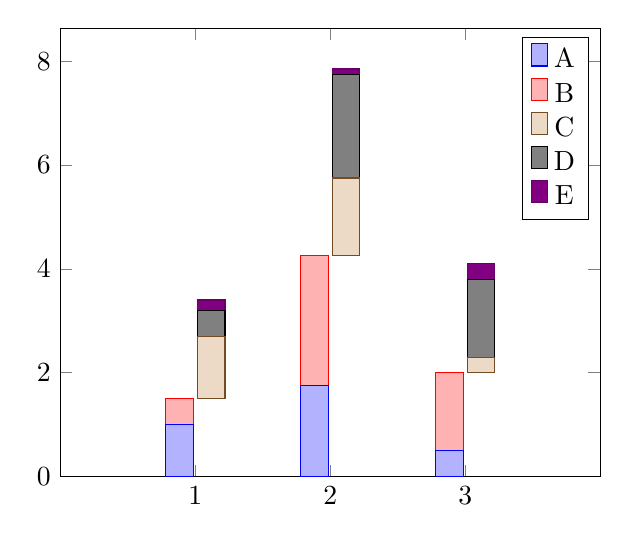
\begin{tikzpicture}
    \begin{axis}[
        ybar stacked,
        xtick=data,
        ymin=0,
        enlarge x limits=0.5,
        legend entries={A,B,C,D,E}
    ]
    \addplot +[bar shift=-.2cm] coordinates {(1,1) (2,1.75) (3,0.5)};
    \addplot +[bar shift=-.2cm] coordinates {(1,0.5) (2,2.5) (3,1.5)};
    
    \resetstackedplots
    
    \addplot  +[bar shift=.2cm]coordinates {(1,1.2) (2,1.5) (3,0.3)};
    \addplot  +[bar shift=.2cm] coordinates {(1,0.5) (2,2) (3,1.5)};
    \addplot  +[bar shift=.2cm] coordinates {(1,0.2) (2,0.1) (3,0.3)};
    \end{axis}
    \end{tikzpicture}

}
\end{figure}


    
\end{document}